%%% template.tex
%%%
%%% This LaTeX source document can be used as the basis for your technical
%%% paper or abstract. Intentionally stripped of annotation, the parameters
%%% and commands should be adjusted for your particular paper - title, 
%%% author, article DOI, etc.
%%% The accompanying ``template.annotated.tex'' provides copious annotation
%%% for the commands and parameters found in the source document. (The code
%%% is identical in ``template.tex'' and ``template.annotated.tex.'')

\documentclass[review]{acmsiggraph}

\TOGonlineid{45678}
\TOGvolume{0}
\TOGnumber{0}
\TOGarticleDOI{1111111.2222222}
\TOGprojectURL{}
\TOGvideoURL{}
\TOGdataURL{}
\TOGcodeURL{}

\title{The Title of Your Paper Goes Here}

\author{Nkenge Wheatland \hspace{10 mm}  
Sophie Joerg
\hspace{10 mm} 
Victor Zordan 
\\UC Riverside
\hspace{16 mm} Clemson University
\hspace{16 mm} UC Riverside}
%\thanks{e-mail:rsmith@gmail.com}
\pdfauthor{}

\keywords{radiosity, global illumination, constant time}

\begin{document}

%% \teaser{
%%   \includegraphics[height=1.5in]{images/sampleteaser}
%%   \caption{Spring Training 2009, Peoria, AZ.}
%% }

\maketitle

\begin{abstract}


\end{abstract}

\begin{CRcatlist}
  \CRcat{I.3.3}{Computer Graphics}{Three-Dimensional Graphics and Realism}{Display Algorithms}
  \CRcat{I.3.7}{Computer Graphics}{Three-Dimensional Graphics and Realism}{Radiosity};
\end{CRcatlist}

\keywordlist

\TOGlinkslist

\copyrightspace



\section{Introduction}
Producing quality whole-body motion involves the movement of the hand in relation to the rest of the body. Using a motion capture system, it is difficult to record the full body of a moving person while also capturing the hand and all of its detail because the whole-body and hand appear at largely different scales.  While it is possible to record a high-resolution capture of the hand through a comprehensive set of markers (typically 13-20 markers), this is best conducted in a small capture region, isolating the motion of the hand.  However, in a larger, full-body capture region the complete set of markers becomes difficult to discern and so this approach is usually abandoned in lieu of the capture of a smaller set of markers (2-6 markers) coupled with a process for reconstructing the full hand animation.  In this paper, we provide a robust technique for the latter that both automatically selects a sparse marker set to record and subsequently produces joint trajectories for a full skeleton from the sparse marker set.  

Specifically, our technique employs a combination of Principle Component Analysis (PCA)~\cite{blahPCA} to construct a low-dimensional representation of the hand data along with a linearly weighted regression (LWR) model to aid in the reconstruction step.  Starting from a reference database that is recorded using a full-resolution marker set, we both determine the best sparse marker set based on the PCA representation from this data as well as use it in the synthesis step with LWR.  We experimented the size of the marker set to record, specifically reduced marker sets of six and three markers and compare our technique with different approaches proposed for selecting the marker, including manual selection as in ~\cite{HoyRyaOSu11} and the use of an representative cluster-based search approach~\cite{KanWheZor12}. In contrast, our technique computes the marker set directly.

For reconstruction, our method employs a smaller number of markers to generate full-hand motion. Based on a test query, we use LWR to build a local model of the full-resolution PCA-version... The results from our reconstructions show that much of the finger specificity needed when communicating with sign language is preserved. We show the power of our technique using American Sign Language (ASL) as a primary testbed along with a few other more generic hand motions, including gesturing and finger-counting.

\section{Related work}

The detailed and subtle motions of fingers are hard to capture. Many approaches have been suggested, each of them having their own advantages and disadvantages. Optical motion capture systems, while being very accurate, require substantial post-processing due to occlusions and mislabelings. CyberGloves \cite{Cyb13} require regular calibrations and do not provide the accuracy needed for our purpose \cite{KahZacKle04}. For image-based systems or systems using depth-data, the hand needs to be in a confined space and the body can not captured synchronously \cite{WanPop09,ZhaChaXu12}. 
% the citation is about cyberglove 2, but I am citing cyberglove 3 previously

Our work focuses on facilitating capturing hand and finger motions together with body motions in a motion capture system. To reach this goal, we investigate the most effective way to capture accurate hand motions using the smallest possible number of markers and an effective reconstruction method. Previous research analyzed finger motions to find correlations between different degrees of freedom. Rijpkema and Girard \shortcite{RijGir91} found that the relationship between the flexion of the distal and the proximal interphalangeal joint (DIP and PIP, respectively) is approximately linear with $DIP=2/3*PIP$. J\"{o}rg and O'Sullivan \shortcite{JoeOSu09} reduce the 50 degrees of freedom of both hands to 15 by eliminating irrelevant and redundant information. These approaches show that finger motions are highly redundant. We take advantage of the correlations between different degrees of freedom of the hand to optimize the capturing and animation of hand motions. 

Principal component analysis (PCA), as a standard technique to analyze and reduce high-dimensional data, has also been used to study finger motions. In Braido and Zhang's study \shortcite{BraZha04}, the two first principal components of a PCA accounted for over 98\% of all variance in the joint angles. However, their motion database did not take into account the thumb and involved only two types of tasks - cylinder grasping and voluntary flexion of individual fingers - which were repeated by different participants. Santello et al. \shortcite{SanFlaSoe98} studied a variety of 57 grasp poses and found that over 80\% of the measured 15 degrees of freedom could be described by their first two principal components. Ciocarlie...
However, all those studies apply to grasps that do not require specific motions from individual fingers. We present a method, which is optimized for American sign language (ASL), which exhibits an impressive dexterity and variety of finger motions. We hypothesize that there is less redundancy in typical finger motions of ASL than in standard grasping motions. 

One of our goals is to determine which is the most effective set of markers for capturing hand motions. Previous work has optimized marker sets for hand motions by choosing markers sets manually and a reconstructing the motions with inverse kinematics \cite{HoyRyaOSu11} or with a brute-force approach that compares the error of similar poses found in a database \cite{KanWheZor13}. 
In a similar manner, but for the full body, Chai and Hodgins, 


%Hoyet...: They find that for many cases a simple 8 marker hand model - one on each fingertip, three of the bases of the thumb, index, and little finger, produces good results. 
%Kang et al. : the best set of six markers includes the fingertips of the index, middle, ring finger as well as three markers on or near the thumb. 
Sign language: ...
Hand low-res: KanWheZor12c, CioGolAll07, ChaPolXin07

Correlations between body and finger motions, in case we manage to include data on the body: MajZorFal06, JoeHodSaf12

Body low-res?: SafHodPol04
Perception?: JoeHodOSu10


\section{Overview}

Our overall technique is divided into two stages: 1) the computation of the sparse marker set; and 2) the reconstruction of the full-resolution, skeleton-driven hand animation from the sparse marker set. 
For our study, we collect full-resolution motion capture data of hand motions in a small capture
area. 
%Our database consists of a total of XXX seconds of American sign language as well as XXX %(a couple of other motions)
%Part of that database is a XXX long sequence consisting of two repetitions of the American sign language alphabet at 120fps (6570 frames) that we use as reference data for our first stage. 
 % are those different versions (different finger poses) or just two repetitions of the ASL alphabet?  
The actor wears 13 small (6mm) markers directly on the hands as well as three markers on the lower forearm. The lower forearm acts as the root link for our hand skeleton with the assumption that these same three markers will appear in full-body captures. 
%The recorded captures act as our database. 
To account for gross body hand motion, marker positions in the database are put into the same coordinate frame by computing the transformation of each marker relative to the root link. Our hand model consists of 18 joints. %describe or include a figure, how are the 18 joints computed based on 13 markers?
For the results in this paper, we construct two such databases, one for sign language and the other freehand gesture data.

In the first phase, we employ the reference data and perform PCA over the markers to derive a rank ordering for the markers based on their influences over the principle components. From this rank-ordered list, we select the top markers to act as our sparse marker set.
For the second phase, reconstruction, we set up a locally weighted regression (LWR) model to map from the sparse marker positions to a set of derived principle components.  In this case, PCA is applied to the joint angles. The LWR model is built for each test query based on the input markers for the query and their proximity to the analogous markers in the reference data after correcting for the lower arm (root) movement.
%
Joint angles for the low dimensional input are then reconstructed by reversing the PCA process from
the principle components computed by the regression to a full set of joint angles. 
%The joint angles are then fed back into the mapping 
%program to animate the hand.

\section{Hand Motion Dimensionality and PCA}

At the core of our technique is the assumption that hand motion is relatively low-dimensional.  Even though a full resolution skeleton of the hand can have several dozen degrees of freedom (DOF), many of the DOFs of the hand show correlations, so that the inherent dimensionality of the hand motions is much lower ~\cite{SanFlaSoe98,BraZha04,JoeOSu09}. In our approach, PCA is used to exploit this low dimensionality as we assume that PCA will allow us to capture the important features of the whole-body hand motion in a small number of principle components.  
%Further, we assume that if we record markers that well-inform these \emph{key} principle components, we can estimate the DOFs of the whole hand.

To support these assumptions, we performed various tests to study the power of PCA for capturing the desired reduced dimensionality of hand motion. 
In Figure~1 below we show that PCA is indeed capable of reducing the dimensionality of the joint angle motion from the database, revealing low average errors for simple reconstruction with reduced numbers of components.  This figure shows erros applied to our ASL database, which represents a diverse expression of poses for the hand.  We see that PCA shows significant reduction in reconstruction error after around 10 components.  While this is larger than reported findings for finger motion, the rich full hand gestures of ASL are still well-represented with a relatively small number of components.
Similar findings are reported using a small set of components from PCA to encapsulate the motion of full-body motion~\cite{SafHodPol04} and our results here support similar observations made over hand motions.


\begin{figure}[!h]
  \centering
  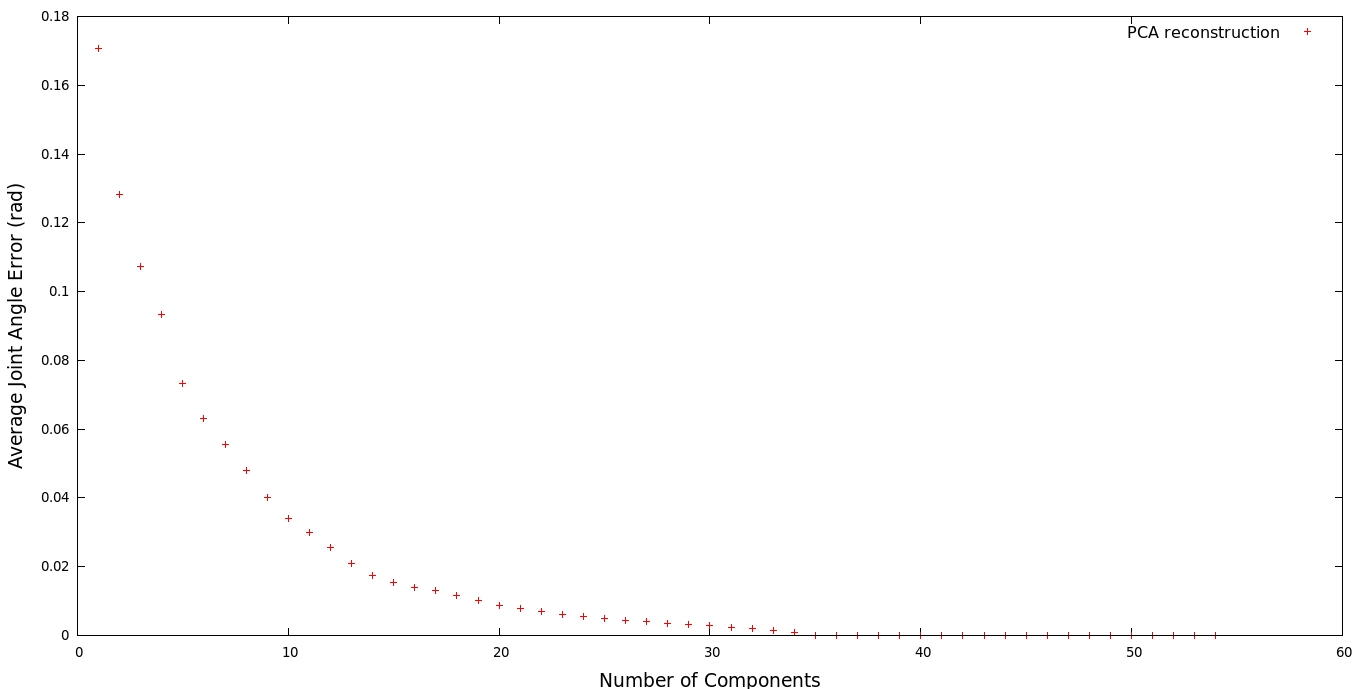
\includegraphics[width=8.3cm]{images/PCA_alphabet_reconstruct.jpg}
  \caption{{\label{fig:pcaError}}Dimensionality reduction for sign language database.  PCA is capable of using as few as ten components with relatively small average errors.}
\end{figure}

\begin{figure}[!h]
  \centering
  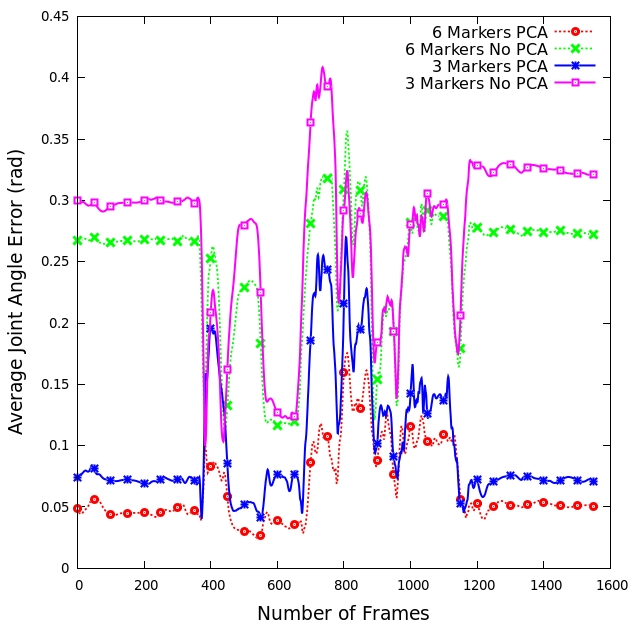
\includegraphics[width=6cm]{images/avgError_6_3_jangles_babySigns1.jpg}
  \caption{{\label{fig:avgError}} Sign language sample motion with and without PCA employed.  Note the
error for six markers without PCA is larger than that of three markers with it. }
\end{figure}

% I know this next bit is weird but the point of the section is to motivate the problem for our domain, 
% and the second figure here is really driving that home

Next, to compare the power of PCA for our particular application we experimented with two reconstruction 
methods with and without PCA. 
The details of the reconstruction appear in Section~6, however, we include the plot in Figure~2 here to support that PCA is very effective in producing higher quality hand motion.
In the figure, we clearly see the benefit of employing PCA as a go-between from markers to joint angles.
When we attempt to reconstruct without it (i.e. markers to joint angles directly) the error remains large
even as the number of markers employed to inform the hand-over process is doubled.



\begin{figure}
  \centering
%  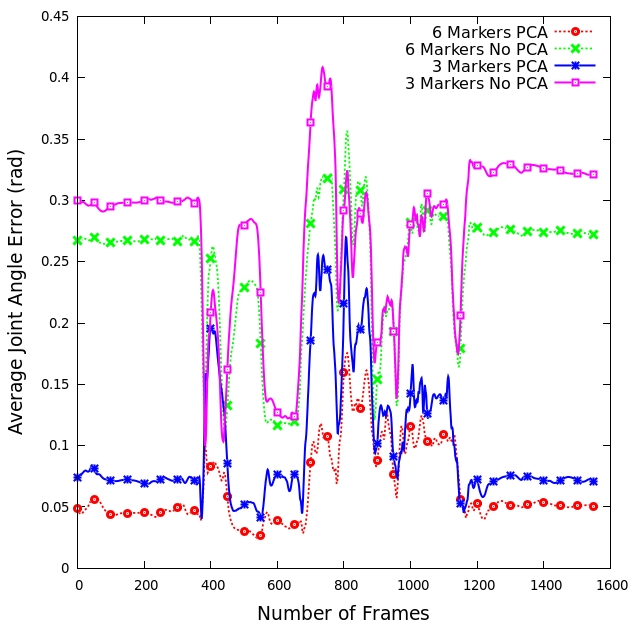
\includegraphics[height=4cm]{images/avgError_6_3_jangles_babySigns1.jpg}
 % \caption{{\label{fig:avgError}}PCA vs. Joint angles.}
\end{figure}



\section{Sparse Marker Selection}
Our method for constructing the sparse marker set exploits the full recordings
that appear in the reference database.  That is, because these recordings 
include a full suite of markers, we can evaluate the value of each marker
in contributing to the whole-hand motion.  A similar approach is described
by Kang et al~\cite{Kang12} but our technique utilizes PCA to compute the markers
directly, as opposed to the exhaustive search proposed by Kang and his
colleagues..

In particular, we conduct PCA over the reference database and, in this case,
PCA is performed with the Cartesian positions of the markers relative
to the root link.  With 13 markers, this leads to a PCA of 39 dimensions.  
In general, PCA produces a covariance matrix and the eigenvectors of this matrix 
create a list of components ordered from most important
to least important.  
%
Each component has 39 coefficients that dictate the influence of each 
marker on that component.  By adding up the contribution of each marker
to all of the components, we can rank-order the influence of the markers on the
full-set of components.  Further, from the eigenvalues, we are given the relative importance
of each principle component with respect to each other.  We can use this importance
as a weighting to bias the components.  Thus, by summing the weighted contribution
of each marker to each of the components, our marker rank ordering can account
for the described bias.

%The marker coeffients are weighted depending 
%on how much the current component contributes to the final PCA reconstruction
%of the database and then summed. Markers with the highest sums are selected to
%be the sparse marker set.

In our results we highlight sparse marker sets of three 
and six markers.
Given the number of markers desired for the sparse set, we select the
set simply as the top markers based the rank-ordering.  We experimented with two methods of
producing this rank-ordering, one with the eigenvalues acting as a weighting bias
and the second treating all of the top-$N$ principle components as equally important and simply
ignoring the remaining components.  Conservatively experimenting with $N$ to be 
between one fourth and three fourths of the full dimensionality, these two approaches 
produced similar results.   However, if we selected $N$ to be the value of the full dimensionality,
we did see reduced quality solutions.  In practice, we employ the eigenvalue weighted ranking for
all results showcased in this paper.  

A nice feature of selecting the marker set in this fashion is that the rank-ordering
simply adds subsequent markers from smaller sets to produce the larger sets.  Thus, the described 
priority ranking reveals which are the definitively \emph{most} influential markers regardless of the
size of the sparse marker set. And so, in practice, adding more
markers for higher quality recordings does not require a complete change of markers, only the
addition of the desired number of markers to the ones employed in the lower quality recording.


%upon the respective marker's contribution to the PCA 
%reconstruction of the reference database.








\section{Reconstruction}

The reconstruction process takes as input a recorded sequence from the sparse marker set.  It then produces joint angle trajectories that estimate the full hand motion.  
%A small number of markers alone cannot produce a fully
%realized hand animation. Therefore, 
To this end, we build a regression model to construct joint angle measurements for a full motion sequence. Specifically, our locally weighted regression (LWR) model maps marker positions in the recorded sequence to principle components. Subsequently, the principle components are converted into joint angles using the covariance matrix from the PCA to produce the final motion.

The LWR model is built for each individual sample, or query, taken from the
recorded sequence.  Through this process,
each instance in the database is weighted and this weighting is used
to bias the model.  The weighting is computed simply as the inverse
of the Euclidean distance from the (root-link corrected) marker positions 
between the query and the samples in the database.  The result
is a regression that places importance on the reference samples
that are close to the test query while also down-weighting the
the influence of reference samples which are more distant
from the query.  For further discussion on this topic, we
refer interested readers to similar efforts with whole-body work~\cite{}.

At run-time, we introduce an input query sequence
recorded from the sparse marker set. The input data is 
put through the regression modeling step to predict the principle components.
To ensure smoothness, the trajectories of the principle components
are filtered before they are converted into joint angles.  In our results, 
we use a cone filter with a size of seventeen, with our sample rate for
the motion recordings set at $120~hz$.  

We also experimented with
filtering the joint angles to produce smoothness, but found more visually 
appealing results when we filtered the principle components.  Our 
assumption for this finding is that the principle components combine
to produce more ``crisp'' poses even when they are filtered while
the joint angle filtering dilutes the unique features of individual
poses over time.  Further study of this phenomena is likely to 
produce interesting findings.


%Reconstruction is completed when PCA process described in 
%Section 4 is reversed, using the newly predicted components
%as input. The result is a full set of joint angles for the
%input motion sequence.


%We test our method on a variety sign language 
%sequences. 

%RESULTS?
% We determine the quality of these animations
% by comparing the reconstructed joint angles to ground truth
% original data. Our method also employs the principle
% component analysis (PCA), and we can access quality by 
% comparing the components of the reconstructed joint angles
% to the components of original joint angles.




\section{Results}
Our primary database is used to reconstruct American Sign Language. 
The database is composed simply of two contiunous
runs of the signs of the letters for the complete 
alphabet, signed by the same actor. We test our method
on various sequences that include words in sign language, most of
which are not included in the database.

For our sparse marker set, we choose to use six markers as our
baseline in order to compare our technique to existing solutions. 
Using the method described in Section 5 to determine 
marker importance, the markers chosen are all of the fingertips
and one on the lower part of the index finger. We also choose a
marker set of three. The markers chosen are the fingertips of the 
middle, ring, and pinky fingers.

Sequences to be recontructed are initially recorded with a full
marker set. Markers not selected for the sparse marker set
are left out of the regression process.

Our method uses regression to predict principle components for
a sequence of motion. In Figure ~\ref{fig:BabySigns_comps}, we compare
the top three predicted components of a sequence of baby sign language
to the components of the original sequence with a full marker set. The
predicted components of six markers and three markers are shown.
Though there are differences, the motion of each component closely
follows that of the ground truth for both marker sets. This can be seen clearly
witha another reconstruced sequence in the video.

We also compare a regression mapping marker positions to principle components to
a regression mapping marker positions directly to joint angles. Figure
~\ref{fig:PCA_noPCA} shows that the average joint angle error for mapping
direclty to joint angles produces a much higher average joint angle error.
The reconstructed hand with six markers fails to reach every distinct pose
in the original animation.

We compare our marker set of six to the markers sets derived from the Manual
Selection Method presented by Hoyet et al. (2011) and the Cluster Pose Error
Method presented by Kang et al.(2012). Using the regression
method, our marker set produces a smaller average joint angle error per frame 
for all of our current sign language tests. The Manual Selection Method's
marker set consistently has the largest joint angle error. Figure
~\ref{fig:3_methods} shows these differences, again using the clip
of baby sign language as an example. The three distinct poses reached
in the baby sign language clip are also shown using the different marker
sets in Figure ~\ref{fig:BabySigns_methods}. Our marker set is consistently
close to the original pose where as
the two other marker fail at achieving at least one pose.\\

\begin{figure}[ht]
  \centering
  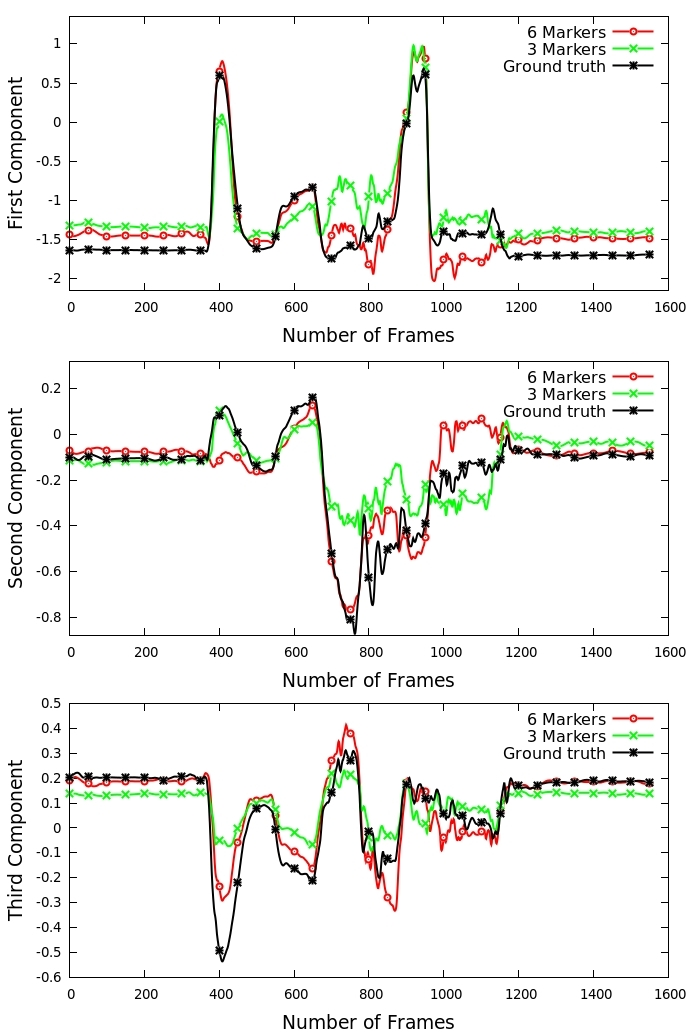
\includegraphics[trim = 28mm 0mm 0mm 0mm,
width=0.45\textwidth]{images/Components_babySigns1.jpg} %width=2.5in
  \caption{Comparison of the components of a reconstructed clip of baby
sign language when using 6 markers and 3 markers. Ground Truth is
the original clip recorded with 13 markers.}
  \label{fig:BabySigns_comps}
\end{figure}

\begin{figure}[ht]
  \centering
  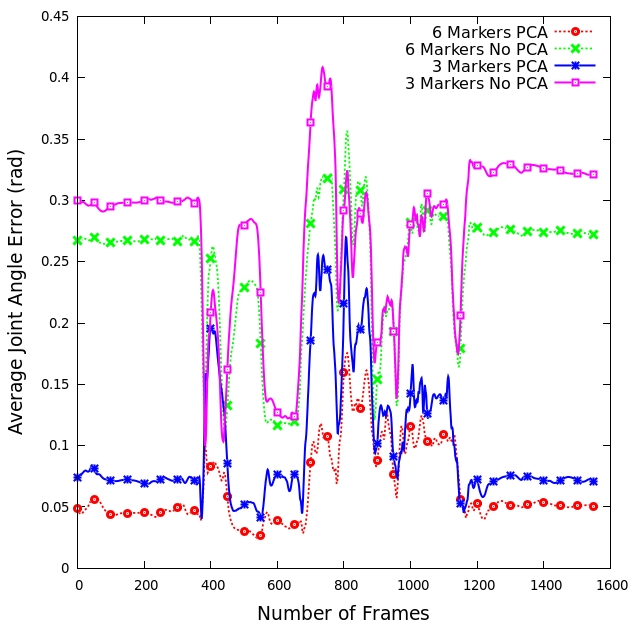
\includegraphics[trim = 28mm 0mm 0mm 0mm,
width=0.45\textwidth]{images/avgError_6_3_jangles_babySigns1.jpg} %width=2.5in
  \caption{Comparison of two regression methods: regression to principle
components and regression to joint angles.}
  \label{fig:PCA_noPCA}
\end{figure}

\begin{figure}[ht]
  \centering
  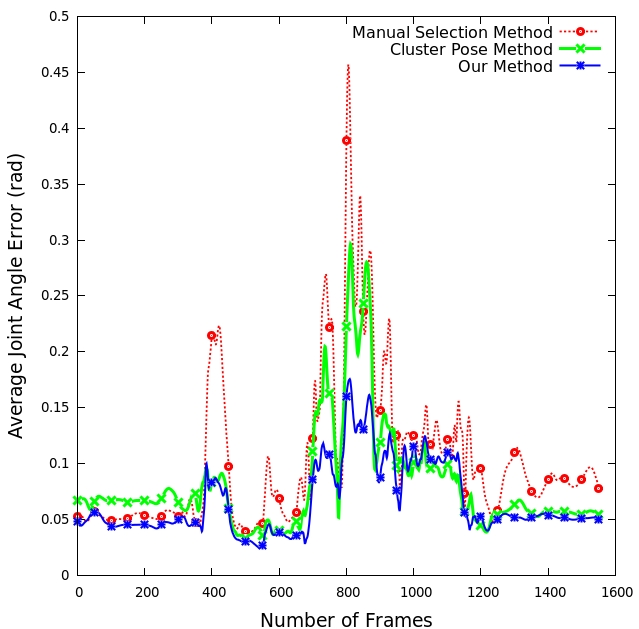
\includegraphics[trim = 28mm 0mm 0mm 0mm,
width=0.45\textwidth]{images/avgError_Marker_sets.jpg} %width=2.5in
  \caption{Comparison of three marker set selection methods that use 6 markers.}
  \label{fig:3_methods}
\end{figure}


\begin{figure}[ht]
  \centering
  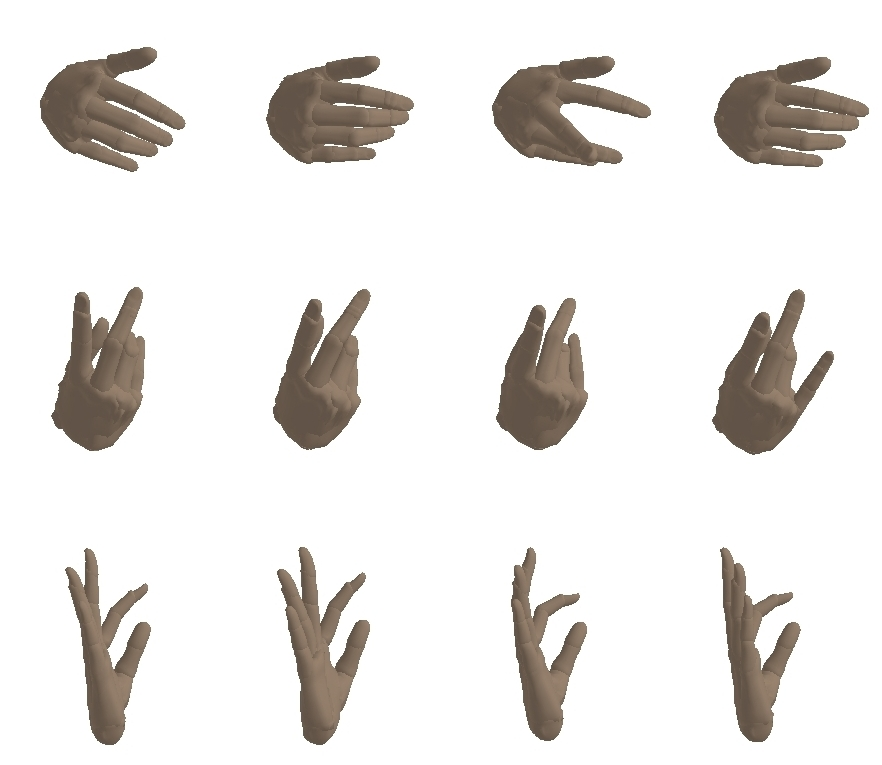
\includegraphics[trim = 28mm 0mm 0mm 0mm,
width=0.45\textwidth]{images/compiled_babySigns1_poses.jpg} %width=2.5in
  \caption{The three distinct poses of the baby sign language clip
reconstructed with the three different marker sets. They are compared to
the original poses.}
  \label{fig:BabySigns_methods}
\end{figure}







\section{Discussion}

When performing the regression we map marker positions to a
certain number of components. We experimented with a smaller 
number of components would produce a better
reconstruction of the joint angle data. We found that mapping
to the full amount of components (54) produces the smallest
average error,
we can map up to 35 components with very little degradation
from a full component set.\\

%Because mapping to a full set of components produces the smallest
%average error, 
We also tested using our locally-weighted
regression model to map marker positions directly to joint angles
represented as Euler angles. The average joint angle error per
frame was very high. This can easily be seen in the animations
produced by the reconstructed joint angles. The hand does not
reach the majority of the poses in the motion. From this we see
that there is a clear benefit to using and producing principle
components to reconstruct the joint angles of the hand over 
mapping directly to joint angles.\\

We also experimented with
 three has a larger average error than the marker
set of six, but still appears to produce reasonable results. We
can see this when looking at the top principle components of the
reconstructed motion and comparing it to the top principle 
components of the original motion. For one sequence of motion,
(in Figure BLAH), the top three components for both the original
motion and the reconstructed motion with 3 markers appear to follow
very similar patterns. Although there is information lost in the
reconstruction, the general pattern of motion is the same.\\

Lastly, we attempt to reconstruct motions that are not sign language
using our alphabet database. The motions include counting and general
gesticulations. While the general poses in the 
sequences appear to be reached, the accuracy of the joint angles
is visibly not as good the sign language reconstructions. It
may be necessary to have a different database to properly reconstruct
these motions.\\


\section{Conclusion}




\iffalse
\begin{equation}
 \sum_{j=1}^{z} j = \frac{z(z+1)}{2}
\end{equation}

\begin{eqnarray}
x & \ll & y_{1} + \cdots + y_{n} \\
  & \leq & z
\end{eqnarray}


\begin{figure}[ht]
  \centering
  \includegraphics[width=1.5in]{images/samplefigure}
  \caption{Sample illustration.}
\end{figure}
\fi


\section*{Acknowledgements}

\bibliographystyle{acmsiggraph}
\bibliography{signPCA}
\end{document}